\chapter{Orthogonality}

\section{Orthogonal Matrices}
\subsection{Definition of Orthogonal Matrices}
In section \ref{vectorops}, we have talked about how two vectors are orthogonal to each other when their dot product is zero. We can extend the concept of orthogonality to matrix. An orthogonal matrix (sometimes called orthonormal) is a matrix whose row vectors (or equivalently column vectors) are of unit length and orthogonal to each other.

\begin{defn}
\label{orthomatrix}
A square matrix
\begin{align*}
P = [\vec{v_1}|\cdots|\vec{v_j}|\cdots|\vec{v_n}] =
\left[
\begin{array}{c}
\vec{w_1} \\
\hline
\cdots \\
\hline
\vec{w_i} \\
\hline
\cdots \\
\hline
\vec{w_n}
\end{array}
\right]
\end{align*}
is said to be orthogonal, if 
\begin{align*}
\vec{v_p} \cdot \vec{v_q} &= 1 & \text{if } p = q \\
\vec{v_p} \cdot \vec{v_q} &= 0 & \text{if } p \neq q
\end{align*}
or 
\begin{align*}
\vec{w_p} \cdot \vec{w_q} &= 1 & \text{if } p = q \\
\vec{w_p} \cdot \vec{w_q} &= 0 & \text{if } p \neq q
\end{align*}
These two requirements are equivalent.
\end{defn}

Vectors in an orthogonal matrix can be generated through Gram-Schmidt orthogonalization and normalization.\\
Short Exercise: Verify that 
\begin{align*}
\begin{bmatrix}
\frac{1}{\sqrt{2}} & \frac{1}{\sqrt{3}} & -\frac{1}{\sqrt{6}} \\
\frac{1}{\sqrt{2}} & -\frac{1}{\sqrt{3}} & \frac{1}{\sqrt{6}} \\
0 & \frac{1}{\sqrt{3}} & \frac{\sqrt{2}}{\sqrt{3}}
\end{bmatrix}
\end{align*}
is an orthogonal matrix.\\
\\
Due to its definition, an orthogonal matrix $P$ has the property $P^TP = PP^T = I$, since the entries of the product are basically dot products of the constituent vectors. We can also say that, $P^TP = PP^T = I$ conversely implies $P$ is orthogonal.
\begin{proper}
\label{orthomatprop}
A matrix $P$ is orthogonal if and only if
\begin{align*}
P^TP = PP^T = I
\end{align*}
\paragraph{Proof} Given that $P = [\vec{v_1}|\vec{v_2}|\vec{v_3}|\cdots]$ satisfies the conditions in Definition \ref{orthomatrix}, then
\begin{align*}
P^T =
\left[
\begin{array}{c}
\vec{v_1}^T \\
\hline
\vec{v_2}^T \\
\hline
\vec{v_3}^T \\
\hline
\cdots
\end{array}
\right]
\end{align*}
and
\begin{align*}
P^T P &=
\begin{bmatrix}
\vec{v_1} \cdot \vec{v_1} & \vec{v_1} \cdot \vec{v_2} & \vec{v_1} \cdot \vec{v_3} & \cdots \\ 
\vec{v_2} \cdot \vec{v_1} & \vec{v_2} \cdot \vec{v_2} & \vec{v_2} \cdot \vec{v_3} & \\ 
\vec{v_3} \cdot \vec{v_1} & \vec{v_3} \cdot \vec{v_2} & \vec{v_3} \cdot \vec{v_3} & \\ 
\vdots & & & \ddots
\end{bmatrix} =
\begin{bmatrix}
1 & 0 & 0 & \cdots \\ 
0 & 1 & 0 & \\ 
0 & 0 & 1 & \\ 
\vdots & & & \ddots
\end{bmatrix}
\end{align*}
The equivalence between $P^TP = I$ and $PP^T = I$ can be derived in a manner similar to the proof in Definition \ref{inverseidentity}. Also, if $P$ is orthogonal, then $P^T$ is orthogonal too.
\end{proper}
By extension, we have the following result.
\begin{proper}
\label{orthoinvT}
If $P$ is an orthogonal matrix, then its inverse is simply its transpose
\begin{align*}
P^{-1} = P^T   
\end{align*}
which also follows from Definition \ref{inverseidentity}.
\end{proper}
Short Exercise: Confirm the properties listed above for the matrix in the last short exercise.

\subsection{Geometric Properties of Orthogonal Matrices}
\label{orthogeometricsub}
All invertible matrices represent some sorts of coordinate transformation as highlighted in Properties \ref{coordinatetrans}. Orthogonal Matrices actually represents a special class of them. Before going into details, we need to start with a simple observation.
\begin{proper}
An orthogonal matrix $P$ has a determinant of either $1$ or $-1$.
\paragraph{Proof} Starting from Properties \ref{orthomatprop}, we have
\begin{align*}
\det(P^TP) &= \det(I) \\
\det(P^T)\det(P) = (\det(P))^2& = 1\\
\det(P) &= \pm 1
\end{align*}
where Properties \ref{properdet} is used.
\end{proper}
Non-zero determinant also confirms that the column vectors in any orthogonal matrix $P$ are linearly independent. Now we are ready to see what kinds of coordinate transformation an orthogonal matrix means.
\begin{thm}
For an orthogonal matrix $P$, if $P$ has a determinant of $1$, then it is a rotation. On the other hand, if $P$ has a determinant of $-1$, then it implies a reflection.
\end{thm}

Depending on the situation, rotation and reflection can be viewed as (a) Rotation and reflection of the vector while keeping the coordinate basis unchanged, or (b) Rotation and reflection of the coordinate system, while keeping the vector in the original place, as the change of coordinate basis mentioned in section \ref{seccoordinatetrans}.

\begin{center}
\begin{tikzpicture}
\draw[->] (0,0)--(3,0) node[right]{$x$};
\draw[->] (0,0)--(0,3) node[above]{$y$};
\draw[red,-stealth] (0,0)--(2,1);
\draw[blue,-stealth] (0,0)--(1,2);
\draw[gray,-stealth] (1.9,1.1)--(1.1,1.9);
\node[below left]{$O$}; 
\end{tikzpicture}
\begin{tikzpicture}
\draw[gray,->] (0,0)--(3,0) node[right]{$x$};
\draw[gray,->] (0,0)--(0,3) node[above](vecu){$y$};
\draw[->] (0,0)--(2.719, 1.268) node[right]{$x'$};
\draw[->] (0,0)--(-1.268, 2.719) node[above](vecv){$y'$};
\draw[Green,-stealth] (0,0)--(2.5,0.5);
\node[below left]{$O$}; 
\pic[draw, ->, "$\theta$", angle eccentricity=1.5] {angle = vecu--0--vecv};
\end{tikzpicture}\\
Left: Case (a), and Right: Case (b), for 2D rotation. 
\end{center}

The construction of rotational or reflectional matrix requires the representation of the new unit axes in the old coordinate system. Just like the change of coordinate basis outlined in Section \ref{seccoordinatetrans}, but with the condition that they are orthogonal to each other. Once they are found, they can be combined column by column to form the transition matrix. For an anti-clockwise (positive) rotation in the right side of the figure above, we have
\begin{align*}
x' &= (\cos \theta) x + (\sin \theta) y \\
y' &= (- \sin \theta) x + (\cos \theta) y
\end{align*}
The corresponding transition matrix is
\begin{align*}
P &= [\hat{x'_s}|\hat{y'_s}] \\
&= \begin{bmatrix}
\cos \theta & -\sin \theta \\
\sin \theta & \cos \theta
\end{bmatrix}
\end{align*}
where the subscript $s$ denotes the standard basis. This matrix can be compared to the one we see in the last chapter when we study the diagonalization variant for complex eigenvalues.\\
\\
If we have an orthogonal matrix $P$, and a vector $\vec{v_0}$ in the standard basis, then doing $\vec{v_n} = P\vec{v_0}$ can be viewed as applying rotation or reflection on the vector $\vec{v_0}$ to produce $\vec{v_n}$ that is still in the standard basis. This is Case (a) we have discussed above. For Case (b), it is the exact opposite. Rotation or reflection of the coordinate system, with the concerned vector $\vec{v_0}$ fixed physically, is achieved by computing $\vec{v_n} = P^{-1}\vec{v_0}= P^T\vec{v_0}$, or taking transpose, $\vec{v_n}^T = \vec{v_0}^T P$. In such situation, the vector is still the same vector in a physical sense, but has its representation expressed in the new coordinate system. Most applications belong to Case (b), thereafter we will limit our discussion to that.\\
\\
However, as a note, these two cases are much related. For example, an anti-clockwise/ positive rotation of a vector in case (a), can be viewed as a clockwise/negative rotation of the coordinate system in case (b), and vice versa.

\begin{exmp}
For a vector $\vec{v_0}$ in the three-dimensional standard basis $B_s$, if the coordinate system undergoes a positive rotation about the $z$-axis by a degree of $\theta$, find its new representation $\vec{v_n}$.

\begin{center}
\begin{tikzpicture}
\node[above left]{$O$}; 
\draw[gray,thick,->] (0,0,0) -- (4,0,0) node[anchor=north east]{$y$};
\draw[thick,->] (0,0,0) -- (0,4,0) node[anchor=north west]{$z = z'$};
\draw[gray,thick,->] (0,0,0) -- (0,0,4) node[anchor=south east](vecu){$x$};
\draw[thick,->] (0,0,0) -- (3.276,0,-2.294) node[anchor=north east]{$y'$};
\draw[thick,->] (0,0,0) -- (2.294,0,3.276) node[anchor=north east](vecv){$x'$};
\pic[draw, ->, "$\theta$", angle eccentricity=1.5] {angle = vecu--0--vecv};
\draw[blue, thick,->] (0,0,0) -- (2,3,2) node[anchor=south west]{$\textbf{v}$};
\end{tikzpicture}     
\end{center}
To construct the rotational matrix, it is required to find the new axes in terms of the old coordinates.
\begin{align*}
& \hat{x_s'} =
\begin{bmatrix}
\cos \theta \\
\sin \theta \\
0
\end{bmatrix},
\hat{y_s'} =
\begin{bmatrix}
-\sin \theta \\
\cos \theta \\
0
\end{bmatrix},
\hat{z_s'} =
\begin{bmatrix}
0 \\
0 \\
1
\end{bmatrix}
\end{align*}
Hence the transition matrix is
\begin{align*}
P =
\begin{bmatrix}
\cos \theta & -\sin \theta & 0 \\
\sin \theta & \cos \theta & 0 \\
0 & 0 & 1
\end{bmatrix}
\end{align*}
For any vector $\vec{v_0} = (x_0,y_0,z_0)^T$ expressed in the standard coordinate basis, the new coordinates after rotation is
\begin{align*}
\vec{v_n} &= P^T\vec{v_0} \\
&=
\begin{bmatrix}
\cos \theta & \sin \theta & 0 \\
-\sin \theta & \cos \theta & 0 \\
0 & 0 & 1
\end{bmatrix}
\begin{bmatrix}
x_0 \\
y_0 \\
z_0
\end{bmatrix} \\
&=
\begin{bmatrix}
(\cos\theta)x_0+(\sin\theta)y_0 \\
(-\sin\theta)x_0+(\cos\theta)y_0 \\
z_0
\end{bmatrix}
\end{align*}
Short Exercise: For the example above, if $(x_0, y_0, z_0)^T = (1,2,3)^T$, the rotation angle is $\theta = \frac{\pi}{8}$, find $\vec{v_n} = (x_n, y_n, z_n)^T$.
\end{exmp}

For successive rotations and reflections, the net transition matrix $P_f$ is produced by taking the product of individual rotational and reflectional matrices each by each. One common convention has the order from right to left, where $\vec{v_n} = (P_n^T\cdots P_3^TP_2^TP_1^T)\vec{v_0}$, and $P_f^T = P_n^T\cdots P_3^TP_2^TP_1^T$. Another equivalent option is to do it from left to right, as in
$\vec{v_n}^T = \vec{v_0}^T(P_1P_2P_3\cdots P_n)$, $P_f = P_1P_2P_3\cdots P_n$.

\begin{exmp}
Find the net transition matrix, if a rotation about $y$-axis about $40$ degree is done first to produce an intermediate coordinate system $x', y', z'$, and then a reflection across the $x'$-$y'$ planeis made to generate the final coordinate system $x'', y'', z''$ (so the new $z''$ axis is the negative of $z'$ axis).\\
\\
The first transition matrix is
\begin{align*}
P_1
&= 
\begin{bmatrix}
\cos(40^\circ) & 0 & \sin(40^\circ) \\
0 & 1 & 0 \\
-\sin(40^\circ) & 0 & \cos(40^\circ)
\end{bmatrix}
\end{align*}
where the readers are encouraged to verify by drawing it out. The second transition matrix is simply
\begin{align*}
P_2
&= 
\begin{bmatrix}
1 & 0 & 0 \\
0 & 1 & 0 \\
0 & 0 & -1
\end{bmatrix}    
\end{align*}
So the net transition matrix is
\begin{align*}
P_f &= P_1P_2 \\
&= 
\begin{bmatrix}
\cos(40^\circ) & 0 & \sin(40^\circ) \\
0 & 1 & 0 \\
-\sin(40^\circ) & 0 & \cos(40^\circ)
\end{bmatrix}
\begin{bmatrix}
1 & 0 & 0 \\
0 & 1 & 0 \\
0 & 0 & -1
\end{bmatrix} \\
&= 
\begin{bmatrix}
\cos(40^\circ) & 0 & -\sin(40^\circ) \\
0 & 1 & 0 \\
-\sin(40^\circ) & 0 & -\cos(40^\circ)
\end{bmatrix}
\end{align*}
\end{exmp}

\section{Orthogonal Diagonalization}

\subsection{Orthogonal Diagonalization for Real Matrices}
\label{orthogonaldiagreal}

Orthogonal diagonalization is a special case of diagonalization, in which the matrix $P$ used to diagonalize another matrix $A$ is an orthogonal matrix. We will discuss the cases for real matrices first.
\begin{defn}
\label{orthodiagonal}
Orthogonal Diagonalization on a real square matrix $A$ is done by an orthogonal matrix $P$ such that $P^{-1}AP = P^TAP = D$ is a diagonal matrix, under the conditions Properties \ref{diagonalize} and Properties \ref{orthoinvT} $P^{-1} = P^T$.
\end{defn}

Not all real square matrices can be orthogonally diagonalized. The requirement is stricter than ordinary diagonalization, but it is a very simple one.
\begin{thm}
\label{symdiag}
A real square matrix $A$ can be orthogonally diagonalized if and only if $A$ is symmetric.
\end{thm}
We also note that matrices in the form $A^TA$ or $AA^T$ can be easily seen to always be symmetric.\\
\\
This theorem has immense implications. As orthogonal diagonalization means that $A$, as an $n \times n$ square matrix, must have $n$ orthogonal eigenvectors as required by Properties \ref{diagonalize} and Definition \ref{orthomatrix}, it leads to a fact that for a matrix $A$, being symmetric guarantees that the eigenvectors are orthogonal. In addition, the eigenvalues are all real. Actually, there is one minor exception, if an eigenvalue for the symmetric matrix is a repeated root of the characteristic equation, then it is possible to obtain eigenvectors that are not orthogonal. However, the problem can be solved by Gram-Schmidt Orthogonalization, as they correspond to the same eigenvalue and it will not affect the overall picture.
\paragraph{Proof} Here is a small proof about the orthogonality of eigenvectors for any symmetric matrix $A$. As defined we have, for two distinct eigenvalues,
\begin{align*}
A\vec{v}_{\lambda_1} &= \lambda_1 \vec{v}_{\lambda_1} \\
A\vec{v}_{\lambda_2} &= \lambda_2 \vec{v}_{\lambda_2}
\end{align*}
Taking the dot product with $\vec{v}_{\lambda_2}$ on the first equation and with $\vec{v}_{\lambda_1}$ on the second one gives
\begin{align*}
(A\vec{v}_{\lambda_1}) \cdot \vec{v}_{\lambda_2} &= \lambda_1 (\vec{v}_{\lambda_1} \cdot \vec{v}_{\lambda_2}) \\
\vec{v}_{\lambda_1} \cdot (A\vec{v}_{\lambda_2}) &= \lambda_2 (\vec{v}_{\lambda_1} \cdot \vec{v}_{\lambda_2})
\end{align*}
But by the symmetry and Properties \ref{dotproper},
\begin{align*}
(A\vec{v}_{\lambda_1}) \cdot \vec{v}_{\lambda_2} = \vec{v}_{\lambda_1} \cdot (A^T\vec{v}_{\lambda_2}) = \vec{v}_{\lambda_1} \cdot (A\vec{v}_{\lambda_2})
\end{align*}
So
\begin{align*}
\lambda_1 (\vec{v}_{\lambda_1} \cdot \vec{v}_{\lambda_2}) &= \lambda_2 (\vec{v}_{\lambda_1} \cdot \vec{v}_{\lambda_2}) \\
(\lambda_1 - \lambda_2)(\vec{v}_{\lambda_1} \cdot \vec{v}_{\lambda_2}) &= 0
\end{align*}
As the eigenvalues are assumed to be distinct, $\lambda_1 - \lambda_2 \neq 0$, and so the dot product $\vec{v}_{\lambda_1} \cdot \vec{v}_{\lambda_2}$ must be zero, the two eigenvectors are orthogonal.

\begin{exmp}
Carry out orthogonal diagonalization on the matrix
\begin{align*}
A =
\begin{bmatrix}
1 & 0 & 0 \\
0 & 2 & 1 \\
0 & 1 & 2
\end{bmatrix}
\end{align*}
First we observe that $A$ is real symmetric and can be orthogonally diagonalized. It can be found that the eigenvectors, after normalization, are
\begin{align*}
&\vec{v_\lambda} = 
\begin{bmatrix}
1 \\
0 \\
0
\end{bmatrix}
,
\begin{bmatrix}
0 \\
-\frac{1}{\sqrt{2}} \\
\frac{1}{\sqrt{2}}
\end{bmatrix}
& \text{for } \lambda = 1 \\
&\vec{v_\lambda} = 
\begin{bmatrix}
0 \\
\frac{1}{\sqrt{2}} \\
\frac{1}{\sqrt{2}}
\end{bmatrix}
& \text{for } \lambda = 3
\end{align*}
Hence we can construct
\begin{align*}
P =
\begin{bmatrix}
1 & 0 & 0 \\
0 & -\frac{1}{\sqrt{2}} & \frac{1}{\sqrt{2}} \\
0 & \frac{1}{\sqrt{2}} & \frac{1}{\sqrt{2}}
\end{bmatrix}
\end{align*}
So that
\begin{align*}
P^TAP &=
\begin{bmatrix}
1 & 0 & 0 \\
0 & -\frac{1}{\sqrt{2}} & \frac{1}{\sqrt{2}} \\
0 & \frac{1}{\sqrt{2}} & \frac{1}{\sqrt{2}}
\end{bmatrix}^T
\begin{bmatrix}
1 & 0 & 0 \\
0 & 2 & 1 \\
0 & 1 & 2
\end{bmatrix}
\begin{bmatrix}
1 & 0 & 0 \\
0 & -\frac{1}{\sqrt{2}} & \frac{1}{\sqrt{2}} \\
0 & \frac{1}{\sqrt{2}} & \frac{1}{\sqrt{2}}
\end{bmatrix} \\
&= 
\begin{bmatrix}
1 & 0 & 0\\
0 & 1 & 0\\
0 & 0 & 3 
\end{bmatrix} = D
\end{align*}
Short Exercise: Confirm the eigenvectors are orthogonal to each other.
\end{exmp}

Another way to see orthogonal diagonalization is to through the so-called spectral decomposition. Rearrangement of the relation gives $A = PDP^T$, if we write $P = [\vec{v}_{\lambda_1}|\vec{v}_{\lambda_2}|\vec{v}_{\lambda_3}|\cdots]$, then expansion gives
\begin{align*}
A &= PDP^T \\
&= [\vec{v}_{\lambda_1}|\vec{v}_{\lambda_2}|\vec{v}_{\lambda_3}|\cdots]
\begin{bmatrix}
\lambda_1 & 0 & 0 & \cdots \\
0 & \lambda_2 & 0 & \\
0 & 0 & \lambda_3 & \\
\vdots & & & \ddots
\end{bmatrix}
\left[
\begin{array}{c}
\vec{v}_{\lambda_1}^T \\
\hline
\vec{v}_{\lambda_2}^T \\
\hline
\vec{v}_{\lambda_3}^T \\
\hline
\cdots
\end{array}
\right] \\
&= 
[\lambda_1\vec{v}_{\lambda_1}|\lambda_2\vec{v}_{\lambda_2}|\lambda_3\vec{v}_{\lambda_3}|\cdots]
\left[
\begin{array}{c}
\vec{v}_{\lambda_1}^T \\
\hline
\vec{v}_{\lambda_2}^T \\
\hline
\vec{v}_{\lambda_3}^T \\
\hline
\cdots
\end{array}
\right] \\
&= \lambda_1 \vec{v}_{\lambda_1}\vec{v}_{\lambda_1}^T + \lambda_2 \vec{v}_{\lambda_2}\vec{v}_{\lambda_2}^T + \lambda_3 \vec{v}_{\lambda_3}\vec{v}_{\lambda_3}^T + \cdots
\end{align*}
It means that in the example above, we can rewrite $A$ into
\begin{align*}
A = (1)
\begin{bmatrix}
1 \\
0 \\
0
\end{bmatrix}
\begin{bmatrix}
1 & 0 & 0
\end{bmatrix}
+(1)
\begin{bmatrix}
0 \\
-\frac{1}{\sqrt{2}} \\
\frac{1}{\sqrt{2}}
\end{bmatrix}
\begin{bmatrix}
0 & -\frac{1}{\sqrt{2}} & \frac{1}{\sqrt{2}}
\end{bmatrix}
+(3)
\begin{bmatrix}
0 \\
\frac{1}{\sqrt{2}} \\
\frac{1}{\sqrt{2}}
\end{bmatrix}
\begin{bmatrix}
0 & \frac{1}{\sqrt{2}} & \frac{1}{\sqrt{2}}
\end{bmatrix}
\end{align*}

\paragraph{Remark} Orthogonal diagonalization is simply a special case for the rotation and reflection of a coordinate system, but acting on a matrix instead of a vector. In general, $P^T AP$ represents rotation and reflection of the matrix $A$.

\subsection{Unitary Diagonalization for Complex Matrices} Now we can generalize the idea of orthogonal diagonalization to complex space. The equivalence of orthogonality for the complex counterpart are unitary matrices.
\begin{defn}
A complex matrix $A$ is said to be unitary if
\begin{align*}
A^*A = AA^* = I
\end{align*}
where the superscript $*$ denotes conjugate transpose.
\end{defn}
The complex equivalent of orthogonal diagonalization is unitary diagonalization.
\begin{defn}
\label{unitarydiag}
A complex square matrix $A$ is said to be unitarily diagonalized if there is a unitary matrix $U$ such that $U^* AU = D$ yields a complex diagonal matrix whose non-zero entries are eigenvalues of $A$.
\end{defn}
This can be compared to Definition \ref{orthodiagonal}. In addition,
\begin{thm}
\label{unitarydiag2}
Unitary orthogonalization is only possible for normal matrices, which has the property
\begin{align*}
A^*A = AA^*    
\end{align*}
and they are not necessarily equal to an identity matrix. Normal matrices always have a full basis of orthonormal eigenvectors, where the complex dot products as defined in Definition \ref{complexdotproduct} are zero between distinct eigenvectors.
\end{thm}
\begin{thm}
For a unitarily diagonalizable matrix $A$, the unitary matrix $U$ required in Definition \ref{unitarydiag} is made up by the column eigenvectors of $A$ mentioned in Theorem \ref{unitarydiag2}, and are unitary in the sense that $U^* U = UU^* = I$.
\end{thm}
Sometimes we refer to the conjugate transpose of a complex matrix $A$ as its Hermitian. However, Hermitian is also used to describe complex square matrix whose conjugate transpose equals to itself.
\begin{defn}
A complex matrix can be said to be Hermitian, if
\begin{align*}
A^* = A
\end{align*}
\end{defn}
In such sense, all Hermitian matrices are also normal matrices, and thus can be unitarily diagonalized. We now see a simple example of unitary diagonalization as the end of this chapter.

\begin{exmp}
Unitarily diagonalize the following matrix.
\begin{align*}
A =
\begin{bmatrix}
1 & 1+\imath \\
1-\imath & 2
\end{bmatrix}
\end{align*}
This can be seen as a Hermitian matrix, and therefore unitary diagonalization is possible. Also notice that a Hermitian matrix has real diagonal entries. The characteristic equation is 
\begin{align*}
(1-\lambda)(2-\lambda) - (1+\imath)(1-\imath) &= 0 \\
(2 - 3\lambda + \lambda^2) - 2 &= 0 \\
\lambda^2 - 3\lambda &= 0 \\
\lambda &= 0 \text{ or } 3
\end{align*}
The eigenvalues being real for an Hermitian matrix is not a mere coincidence. In fact, it is an extension on the notes included for Theorem \ref{symdiag}. The eigenvectors can be computed to be $(-1-\imath, 1)^T$ for $\lambda = 0$ and $(1+\imath, 2)^T$ for $\lambda = 3$. After normalization, they are $\frac{1}{\sqrt{3}}(-1-\imath, 1)^T$ and $\frac{1}{\sqrt{6}}(1+\imath, 2)^T$ respectively. Now define
\begin{align*}
U =
\begin{bmatrix}
\frac{-1-\imath}{\sqrt{3}} & \frac{1+\imath}{\sqrt{6}} \\
\frac{1}{\sqrt{3}} & \frac{\sqrt{2}}{\sqrt{3}}
\end{bmatrix}
\end{align*}
Then the unitary diagonalization has the form of
\begin{align*}
U^* AU &= D \\
\begin{bmatrix}
\frac{-1+\imath}{\sqrt{3}} & \frac{1}{\sqrt{3}} \\
\frac{1-\imath}{\sqrt{6}} & \frac{\sqrt{2}}{\sqrt{3}}
\end{bmatrix}
\begin{bmatrix}
1 & 1+\imath \\
1-\imath & 2
\end{bmatrix}
\begin{bmatrix}
\frac{-1-\imath}{\sqrt{3}} & \frac{1+\imath}{\sqrt{6}} \\
\frac{1}{\sqrt{3}} & \frac{\sqrt{2}}{\sqrt{3}}
\end{bmatrix}
&=
\begin{bmatrix}
0 & 0 \\
0 & 3
\end{bmatrix}
\end{align*}
\end{exmp}

\section{Exercise}

\begin{Exercise}
Determine if the following matrices are orthogonal. If so, also determine if they represent rotation or reflection.
\begin{enumerate}[label=(\alph*)]
\item $\begin{bmatrix}
\frac{1}{\sqrt{2}} & 0 & \frac{1}{\sqrt{2}}\\
\frac{3}{2\sqrt{6}} & \frac{1}{2} & -\frac{3}{2\sqrt{6}}\\
-\frac{1}{2\sqrt{2}} & \frac{\sqrt{3}}{2} & \frac{1}{2\sqrt{2}}
\end{bmatrix}$
\item $\begin{bmatrix}
-\frac{\sqrt{3}}{2} & \frac{1}{2} & 0\\
\frac{1}{4} & \frac{\sqrt{3}}{4} & -\frac{\sqrt{3}}{2}\\
\frac{\sqrt{3}}{4} & \frac{3}{4} & \frac{1}{2}
\end{bmatrix}$
\item $\begin{bmatrix}
1 & 3 & 2\\
2 & 1 & 3\\
0 & 1 & 0
\end{bmatrix}$
\item $\begin{bmatrix}
\sqrt{7} & 0 & 0\\
0 & \sqrt{5} & 0\\
0 & 0 & 1
\end{bmatrix}$
\end{enumerate}
\end{Exercise}

\begin{Exercise}
Represent the following operations on a three-dimensional $xyz$ coordinate system by a transitional matrix $P$. State clearly the relationship between the vectors in old and new coordinate system ($\vec{v_0}$ and $\vec{v_n}$), as well as the matrix $P$.
\begin{enumerate}[label=(\alph*)]
\item Rotation about the z-axis (x-axis and y-axis revolving around the z-axis) counter-clockwise by 45 degrees,
\item Reflection of the x-axis across the y-z plane and subsequently rotation about the intermediate y-axis counter-clockwise by 30 degrees,
\item Rotation about the y-axis clockwise by 45 degrees, and then rotation about the new z-axis counter-clockwise by 60 degrees.
\end{enumerate}
It is emphasized that the order of operations is important.
\end{Exercise}

\begin{Exercise}
For the symmetric matrix 
\begin{align*}
\begin{bmatrix}
1 & a & a\\
a & 5 & 3\\
a & 3 & 5
\end{bmatrix}
\end{align*}
It is given that one of the eigenvalues is zero and the product of other two eigenvalues is $18$. Using the knowledge that the trace and characteristic polynomial are invariants, i.e. remains unchanged after diagonalization. Find 
\begin{enumerate}[label=(\alph*)]
\item The two remaining eigenvalues,
\item The possible values of $a$,
\item For every possible case, find the eigenvector corresponding to the eigenvalue of zero, then carry out orthogonal diagonalization.
\end{enumerate}
\end{Exercise}

\begin{Exercise}
Orthogonally diagonalize the following matrix, if possible.
\begin{enumerate}[label=(\alph*)]
\item $\begin{bmatrix}
7 & 8 & 10\\
1 & 6 & 3\\
5 & 1 & 2
\end{bmatrix}$
\item $\begin{bmatrix}
2 & 0 & 1\\
0 & 2 & 1\\
1 & 1 & 1
\end{bmatrix}$
\item $\begin{bmatrix}
3 & 1 & 1\\
1 & 3 & 1\\
1 & 1 & 3
\end{bmatrix}$
\end{enumerate}
\end{Exercise}

\begin{Exercise}
In continuum mechanics, the stress tensor is a symmetric matrix (to be more accurate, a tensor) describing the stress inside a material at a point. The eigenvalues for the stress tensor are called principal stresses and the corresponding eigenvectors are named principal axes. For the stress tensor
\begin{align*}
\sigma = 
\begin{bmatrix}
4 & 2\\
2 & 1
\end{bmatrix}
\end{align*}
(in MPa), find its principal stresses and principal axes. (Calculus required) Also, find the maximum possible value attained by the shear stress $\sigma_{12} = \sigma_{21} = \sigma_{s}$ if the stress tensor undergoes rotation.
\end{Exercise}

\begin{Exercise}
Show that the matrix below is Hermitian and unitarily diagonalize it.
\begin{align*}
A &=
\begin{bmatrix}
1 & -\imath & 0 \\
\imath & 2 & 1+\imath \\
0 & 1-\imath & 3 
\end{bmatrix}
\end{align*}
\end{Exercise}

\begin{Exercise}
Hooke's law states that the force acting on a mass by spring is given by $F = -kx$ where $k$ is the spring constant and $x$ is the displacement (extension or compression) from equilibrium position. By considering Newton's second law, $F = ma$, we have
\begin{equation*}
ma = m\frac{d^2x}{dt^2} = -kx\text{ and hence }x'' = \frac{d^2x}{dt^2} = -\frac{k}{m}x
\end{equation*}
The general solution is
\begin{equation*}
x = C\cos(\omega t - \theta)
\end{equation*}
where $\omega = \sqrt{\frac{k}{m}}$ and $C$, $\theta$ are some arbitrary constants to be determined from the initial condition. Consider the situation  shown in the figure below. Find the two equations describing motions of the two masses $m_1, m_2$ respectively, in terms of the displacements $\textbf{x} = (x_1, x_2)^T$, and re-written them into matrix form. Carry out orthogonal diagonalization to simplify the equations and find the general solutions for the motions.
\begin{center}
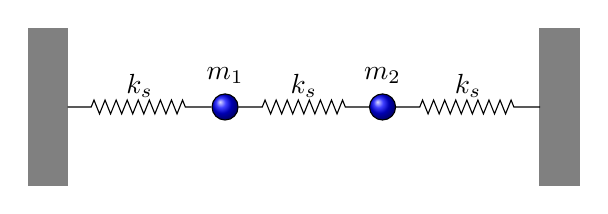
\begin{tikzpicture}
[wall/.style = {gray,fill=gray},
mass/.style = {draw,circle,ball color=blue},
spring/.style = {decorate,decoration={zigzag, pre length=.3cm,post length=.3cm,segment length=#1}},]
\draw[wall] (-.5,-1) rectangle (0,1);
\coordinate (l) at (0,0);
\node[mass,label={above:$m_1$}] (m1) at (2,0) {};
\node[mass,label={above:$m_2$}] (m2) at (4,0) {};
\coordinate (r) at (6,0);
\draw[wall] (6,-1) rectangle (6.5,1);

\draw[spring=4pt] (l) -- node[above] {$k_s$} (m1);
\draw[spring=4pt] (m1) -- node[above] {$k_s$} (m2);
\draw[spring=4pt] (m2) -- node[above] {$k_s$} (r);
\end{tikzpicture}  
\end{center}
\end{Exercise}